\documentclass[12pt,a4paper,oneside]{ctexart}

\usepackage{amsmath,amsthm,amssymb,appendix,bm,graphicx,hyperref,mathrsfs}
\usepackage{geometry,pifont,ctex}
\usepackage{float}  % 图片位置设置
\usepackage{listings} % 插入代码块
\usepackage{color}
\usepackage{hyperref}


\usepackage{enumitem}
\setlist[itemize]{itemsep=1.6pt, topsep=4pt, parsep=0pt, partopsep=0pt} % itemize 行距
\geometry{left=2.54cm,right=2.54cm,top=3.18cm,bottom=3.18cm}
\linespread{1.5}

% 标题、作者、日期
\title{RISC-V 流水线处理器 \\   
        \large{—— 2023年秋季学期《计算机组成原理》大实验报告}}
\author{
    Group 19
}

\date{\kaishu{\today}}

\begin{document}
% 标题
\maketitle
\newpage
% 目录
\tableofcontents
\newpage


\section{实验目标}

\begin{itemize}
    \item 深入理解流水线结构计算机指令的执行方式,掌握流水处理器的基本设计方法。
    \item 深入理解计算机的各部件组成及内部工作原理。
    \item 加深对于 RV32I 指令集的理解。
    \item 掌握计算机外部输入输出的设计。
    \item 提高硬件设计和调试的能力。
\end{itemize}


\section{CPU 结构设计}
% 实验报告要求1:给出 CPU 的结构图。简述每个功能模块的功能。
\begin{figure}[ht]
    \centering
    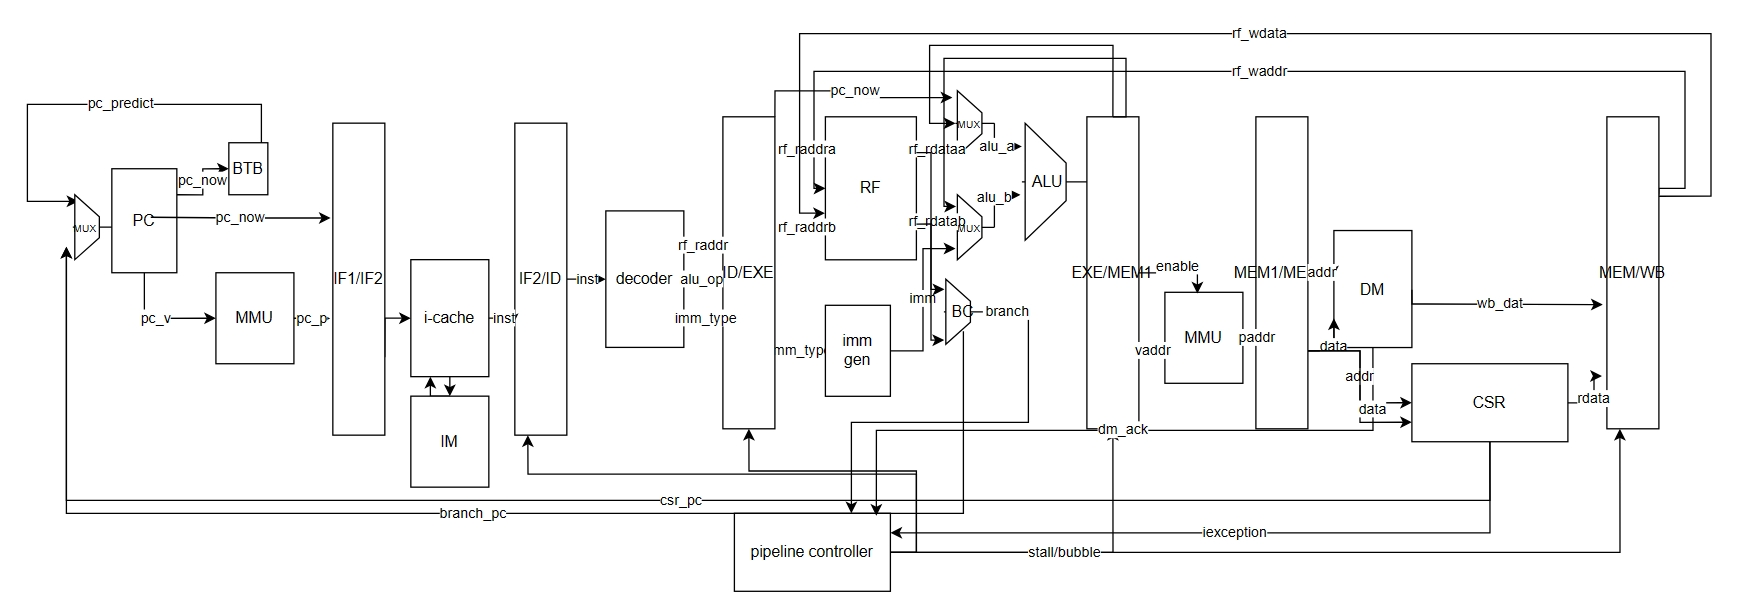
\includegraphics[scale=0.26]{assets/cpu.png}
    \caption{CPU 结构与数据通路图}
    \label{fig:cpu}
\end{figure}

采用七级流水线设计,将 IF 和 MEM 阶段拆分,分为 IF1、IF2、ID、EXE、MEM1、MEM2、WB 七个阶段。
\begin{itemize}
    \item IF1 阶段通过 MMU 将虚拟的指令地址转换为物理地址,使用 BTB 进行分支预测,并完成 PC 的更新。
    \item IF2 阶段根据 PC 从内存读取指令,并实现了指令缓存模块 icache。
    \item ID 阶段完成指令的译码。
    \item EXE 阶段负责从寄存器堆读取、完成 ALU 的计算以及条件跳转指令的比较运算。
    \item MEM1 阶段将虚拟的访存地址通过 MMU 转换为物理地址。
    \item MEM2 阶段负责内存的写入,CSR 寄存器的读写和异常处理也在这一阶段完成。
    \item WB 阶段进行寄存器堆的写入操作。
\end{itemize}

\section{实验内容}
% 实验报告要求2:简述数据前传部分的实现逻辑。并给出数据冲突的例子(假设 IF 段和 MEM 段功能可以在 1 周期内完成),以及对应关键信号的波形图。

% 实验报告要求3:对于每个实现的扩展功能,简要介绍功能是如何实现的。给出功能实现原理波形图,以及上板实验的截图 / 性能数据对比。
在大实验中,本组完成的内容如下:
\begin{itemize}
    \item 功能类 \begin{itemize}
        \item 异常与中断
        \item 虚拟内存与页表
        \item S 态与 uCore
    \end{itemize}
    \item 性能类 \begin{itemize}
        \item 指令缓存
        \item 分支预测
        \item TLB
        \item 提高流水线级数(7 级)
    \end{itemize}
    \item 外设类 \begin{itemize}
        \item VGA
        \item Flash
    \end{itemize}
\end{itemize}

我们实现的 RISC-V 处理器支持 RV32I 的所有指令,能够运行三个版本的监控程序以及uCore 操作系统,并可以通过 VGA 播放视频。

实验分工为:孙维泽完成中断异常及各内核态、uCore 调试;陈鑫圣完成页表及虚拟地址转换、TLB、uCore 调试;张凯文完成指令缓存、分支预测、外设。

实验基于孙维泽 Lab 6 的流水线处理器框架(其中 SRAM 控制器使用陈鑫圣 Lab 6 的版本)。

\subsection{异常与中断}

\subsubsection{CSR 寄存器读写}

实现了实验文档要求的所有 CSR 寄存器,其中由于 sstatus、sie 和 sip 寄存器的字段均为 mstatus、mie、mip 寄存器的子集,因此没有单独实现这些 S 态寄存器,而是将其读写映射到对应的 M 态寄存器上。

CSR 寄存器的读写均在 MEM2 阶段完成,并针对不同的 CSR 寄存器实现了不同的读写权限。当流水线中存在 CSR  读写指令时,我们选择暂停流水线,保证在流水线中至多只有 1 条 CSR 读写指令。对于写 CSR 指令可能出现的数据冲突,可以通过已有的数据旁路解决。

\subsubsection{异常中断处理}

在各个流水段都会产生异常信号,比如:IF1 阶段会产生 Instruction address misaligned、Instruction  page fault、Instruction access fault 异常。所有的异常信号汇总到 MEM2 阶段,异常处理模块会根据输入的信号和当前的特权态,进行相应的异常处理。实现了 medeleg 寄存器,可以根据其判断是否进行异常委托,从而决定在 M 态或 S 态进行异常处理。

当发生异常时,根据异常的类型及来源设置 xcause ,并对 xtval 进行相应设置,将当前的 PC 保存到 xepc,将当前特权等级保存到 mstatus.xpp,将当前的 mstatus.xie 保存到 mstatus.xpie,并将 mstatus.xie设置为 0 以禁用中断。同时,模块会给出跳转信号,更新 PC 值并由流水线控制器冲刷当前的流水线。此外,当 MEM2 阶段检测到发生异常时,会阻止当前阶段的内存写入,以保证 CPU 的正确性。

中断方面,实现了 mtime 和 mtimecmp 寄存器,处理模块会根据 mtime 和 mtimecmp 的比较结果 设置 mip 寄存器的 mtip 字段,以支持对时钟中断的判断。当发生时钟中断时,为了不受气泡影响,我们选择将中断发生后第一条进入 MEM2 阶段的非空指令作为中断返回的 PC 值。
 
\subsection{虚拟内存与 TLB}

虚拟内存机制的设计对应的模块为 \texttt{mmu},在 CPU 结构中为取指和访存阶段各例化一个 \texttt{mmu}(在 IF1, MEM1 流水段)。

\texttt{mmu} 模块为一个状态机。首先判断是否直接映射,如果是则直接输出结果,否则进入地址翻译。地址翻译时,先判断 TLB 是否 hit,(即是否存在相应表项),如果存在则直接输出,否则进入第一级页表的读取,读取完毕后判断 是否有异常(如有,则中止翻译,并发出 page fault 或 access fault 信号),然后进行第二级页表的读取(与第一级页表相似)。如果没有任何异常,则输出结果并将结果写入 TLB。

TLB 设计为直接映射,容量为 32 项。相对于没有 TLB 的版本,在前 3 个测例上性能提升到 8 倍左右,在第 4、5 个测例上性能提升到 4.4 倍、5.2 倍左右。参见 \ref{performance}。
% 7.997, 7.993, 8.000, 4.415, 5.157

为让虚拟地址转换和实际数据的读写更好地解耦,同时提升性能(相对于在一个流水段进行地址翻译和数据读写),我们将 5 段流水线升级为 7 段流水线,将 IF 和 MEM 阶段拆成两部分,第一阶段(IF1, MEM1)进行地址翻译,第二阶段(IF2,MEM2)进行实际的数据读写。为此,我们重新设计部分数据通路和冲突处理,详见 \ref{pipeline-control} 流水线控制信号。

\subsection{数据旁路}

对于 load-use 之外的数据冲突,都可以用数据旁路来解决,相应代码如下(在 \texttt{EXE} 模块中)。

\begin{lstlisting}[
    numbers=left,
    frame=single,           % 添加边框
    basicstyle=\fontsize{6}{10}\selectfont, % 设置全局字号
    lineskip=4pt,           % 设置行距
    tabsize=4,              % 设置制表符的宽度为4个空格
    % xleftmargin=15pt,       % 设置左侧缩进的距离为15pt
    caption={数据旁路实现代码} % 标题
] 
    assign rf_rdata_a_forwarded = (exe_mem1_rf_waddr_i != 0  && (exe_mem1_rf_waddr_i  == rf_raddr_a_i)) ? exe_mem1_alu_result_i :
                                  (mem1_mem2_rf_waddr_i != 0 && (mem1_mem2_rf_waddr_i == rf_raddr_a_i)) ? mem1_mem2_rf_wdata_i :
                                   rf_rdata_a_i;
    assign rf_rdata_b_forwarded = (exe_mem1_rf_waddr_i != 0  && (exe_mem1_rf_waddr_i  == rf_raddr_b_i)) ? exe_mem1_alu_result_i :
                                  (mem1_mem2_rf_waddr_i != 0 && (mem1_mem2_rf_waddr_i == rf_raddr_b_i)) ? mem1_mem2_rf_wdata_i :
                                   rf_rdata_b_i;
    /* MEM1-EXE, MEM2-EXE 的指令都不是 load-use 关系,这点由 pipeline_controller 保证 */
    /* 对于 WB 正在写寄存器的情况,已经在 regfile 中实现了相应的旁路 */
    /* 目前的实现中,如果有 CSR 指令进入流水线,则暂暂停 IF1,即 CSR 指令后不会再有其它任何指令,
       所以不需要考虑 CSR 读写指令修改 rs1, rs2 的情况 */
\end{lstlisting}

在我们的实现中,对 CSR 指令进行了特别处理:如果有 CSR 指令进入流水线,则暂停 IF1(参见 \ref{pipeline-control}),即 CSR 指令后不会再有其它任何指令,所以不需要考虑 CSR 读写指令修改 rs1, rs2 的情况。

一个例子如下
\begin{lstlisting}[
    numbers=left,
    frame=single,           % 添加边框
    basicstyle=\fontsize{6}{10}\selectfont, % 设置全局字号
    lineskip=4pt,           % 设置行距
    tabsize=4,              % 设置制表符的宽度为4个空格
    % xleftmargin=15pt,       % 设置左侧缩进的距离为15pt
    caption={数据旁路实现代码} % 标题
] 
    addi t0, zero, 0     # loop variable      # [00] 00000293
    addi t1, zero, 100   # loop upper bound   # [04] 06400313
    addi t2, zero, 0     # sum                # [08] 00000393
loop:
    addi t0, t0, 1                            # [0c] 00128293
    add t2, t0, t2                            # [10] 007283B3
    beq t0, t1, next # i == 100?              # [14] 00628463
    beq zero, zero, loop                      # [18] fe000ae3
\end{lstlisting}

\texttt{loop} 后的前两条指令会有数据冲突,但是加入数据旁路后可以解决。从仿真中可以看到,确实没有导致额外的暂停和气泡。

\begin{figure}[H]
    \centering
    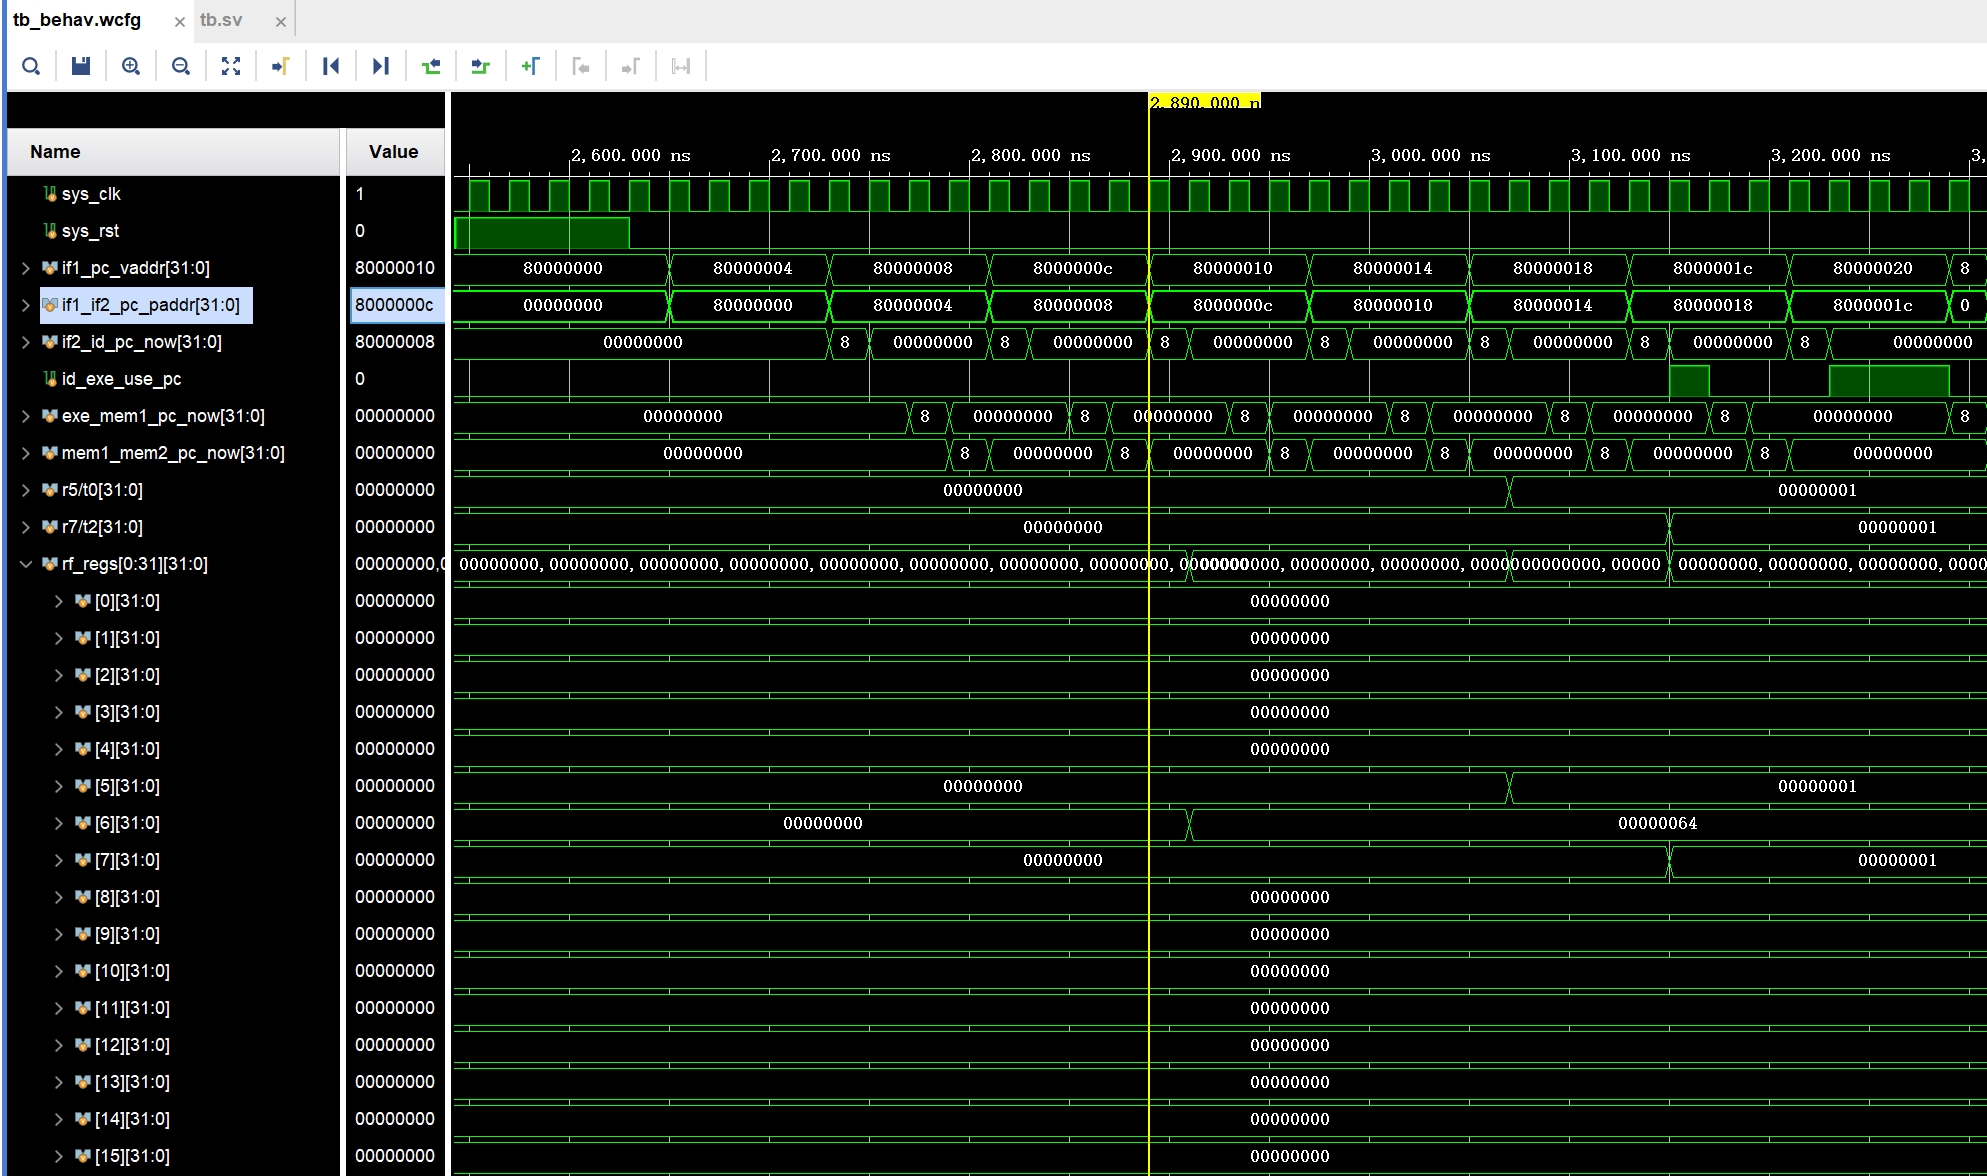
\includegraphics[scale=0.18]{assets/data-forwarding.png}
    \caption{数据旁路}
    \label{fig:data-forwarding}
\end{figure}

\subsection{指令缓存}
在IF2阶段加入icache模块,根据直接映射方式存储指令缓存,在取指令时统一将PC传给icache,若命中则直接返回缓存的指令,否则通过总线请求得到指令,并更新缓存表。

\subsection{分支预测}
使用两位预测机制、直接映射的BTB缓存表,两位中高位为1则有效,否则无效,且表中仅对分支指令存储分支跳转信息。根据当前PC预测下一PC,命中且有效则返回预测值,否则返回PC+4;根据EXE阶段返回的跳转结果更新表项,跳转成功则有效位+1(11封顶不再加),否则-1(00封顶不再减),若遇到跳转指令单但当前PC不在表中则存储。

\subsection{流水线控制信号} \label{pipeline-control}

流水线中各流水段控制信号如下表。其中某个流水段为 \texttt{Stall} 表示该流水段的输出保持不变,为 \texttt{Bubble} 表示该流水段的输出为气泡(相当于 \texttt{nop} 指令),

\begin{table}[H]
\caption{流水线控制信号}
\begin{tabular}{lllllll}
 & IF1 & IF2 & ID & EXE & MEM1 & MEM2 \\
 \hline
MEM2读写 & Stall & Stall & Stall & Stall & Stall & Bubble \\
CSR跳转且IF1/IF2/MEM1读写 & Stall & Stall & Stall & Stall & Stall & Bubble \\
CSR Branch & Bubble & Bubble & Bubble & Bubble & Bubble & Bubble \\
MEM1读写 & Stall & Stall & Stall & Stall & Bubble &  \\
普通跳转且IF1/IF2读写 & Stall & Stall & Stall & Bubble &   &   \\
普通跳转 & Bubble & Bubble & Bubble &   &   &   \\
Load relate & Stall & Stall & Bubble &   &   &   \\
fence.i & Stall & Bubble &   &   &   &   \\
CSR读写 & Stall & Bubble &   &   &   &   \\
IF2读写 & Stall & Bubble &   &   &   &   \\
sfence.vma且IF1读写 & Stall & Bubble &   &   &   &   \\
sfence.vma & Bubble &   &   &   &   &   \\
IF1读写 & Bubble &   &   &   &   &   \\
\end{tabular}
\end{table}

\section{效果展示}
\subsection{性能对比}
各个版本在测例上的运行时间如下表,相应的版本已在仓库中打上 tag。除最后一列以外,其余测试均在 10MHz 时钟频率下测得,从左向右为递进关系,即右侧的测试中包含左侧的所有优化。

\begin{table}[H] \label{performance}
\caption{性能对比(单位:s)}
\begin{tabular}{lllllllll}
 & Baseline & 指令缓存 & 数据旁路 & 分支预测 & MMU & TLB & 50MHz \\
 \hline
1PTB & 161.100 & 46.973 & 46.985 & 33.586 & 268.435 & 33.556 & 6.713  \\
2DCT & 80.531 & 67.111 & 21.810 & 18.454 & 147.646 & 18.471 & 3.695  \\
3CCT & 187.908 & 67.137 & 67.109 & 26.837 & 214.757 & 26.846 & 5.398  \\
4MDCT & 181.198 & 104.024 & 80.543 & 73.825 & 355.675 & 80.564 & 16.155  \\
UTEST\_PUTC & 8.178 & 6.413 & 2.517 & 2.300 & 15.720 & 3.048 & 0.474
\end{tabular}
\end{table}

\subsection{运行 uCore}

\begin{figure}[H]
    \centering
    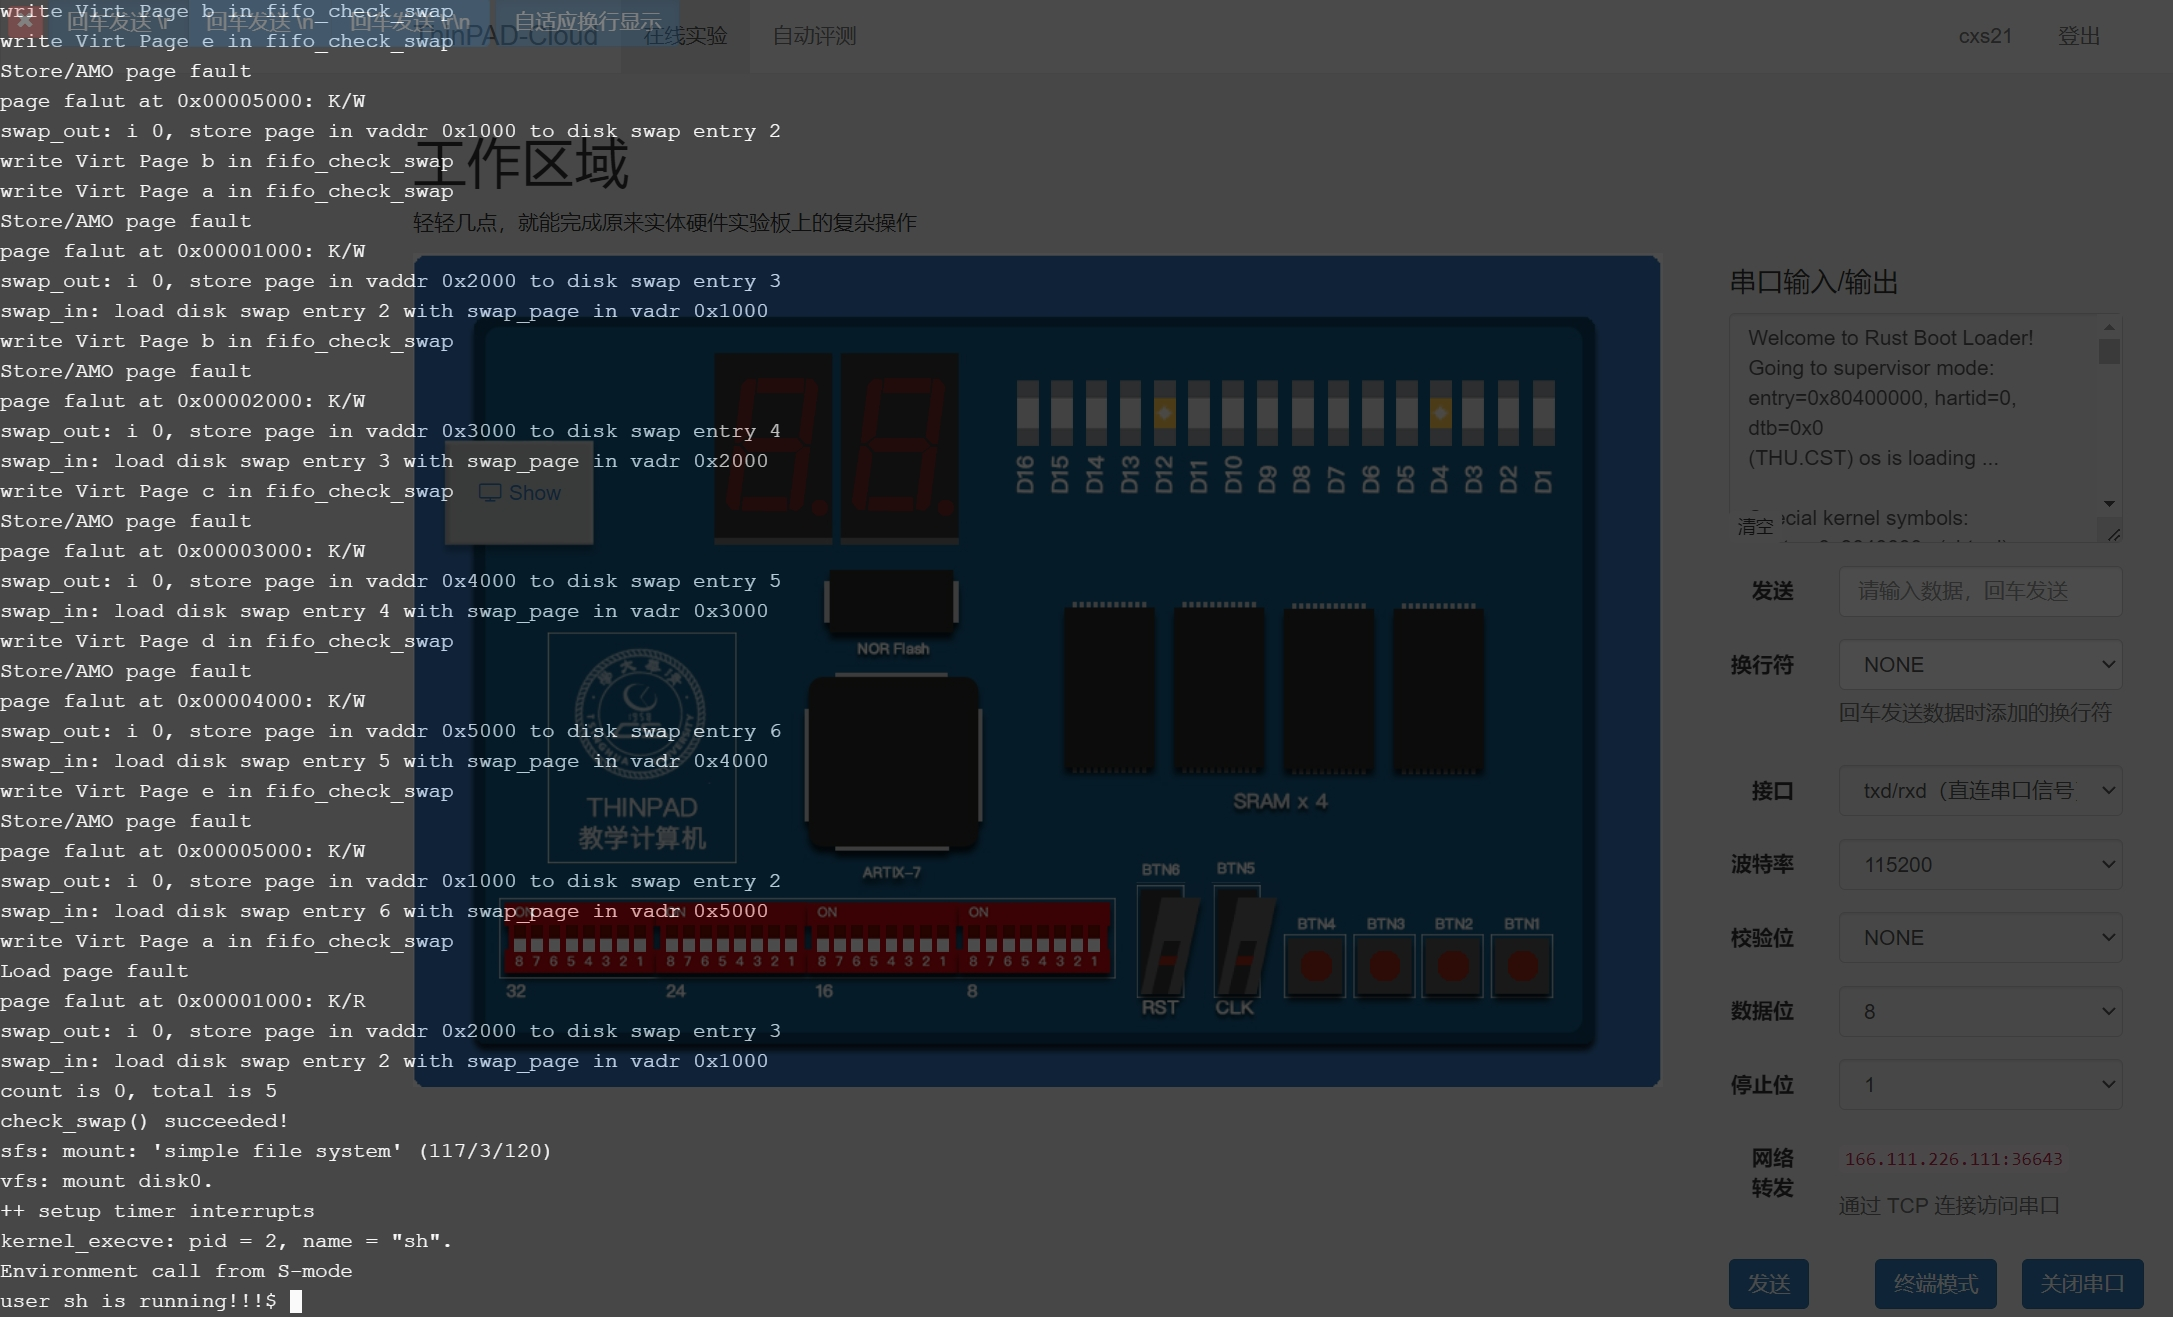
\includegraphics[scale=0.18]{assets/ucore_init.png}
    \caption{uCore 运行截图 - 初始化}
    \label{fig:uCore_init}
\end{figure}

\begin{figure}[H]
    \centering
    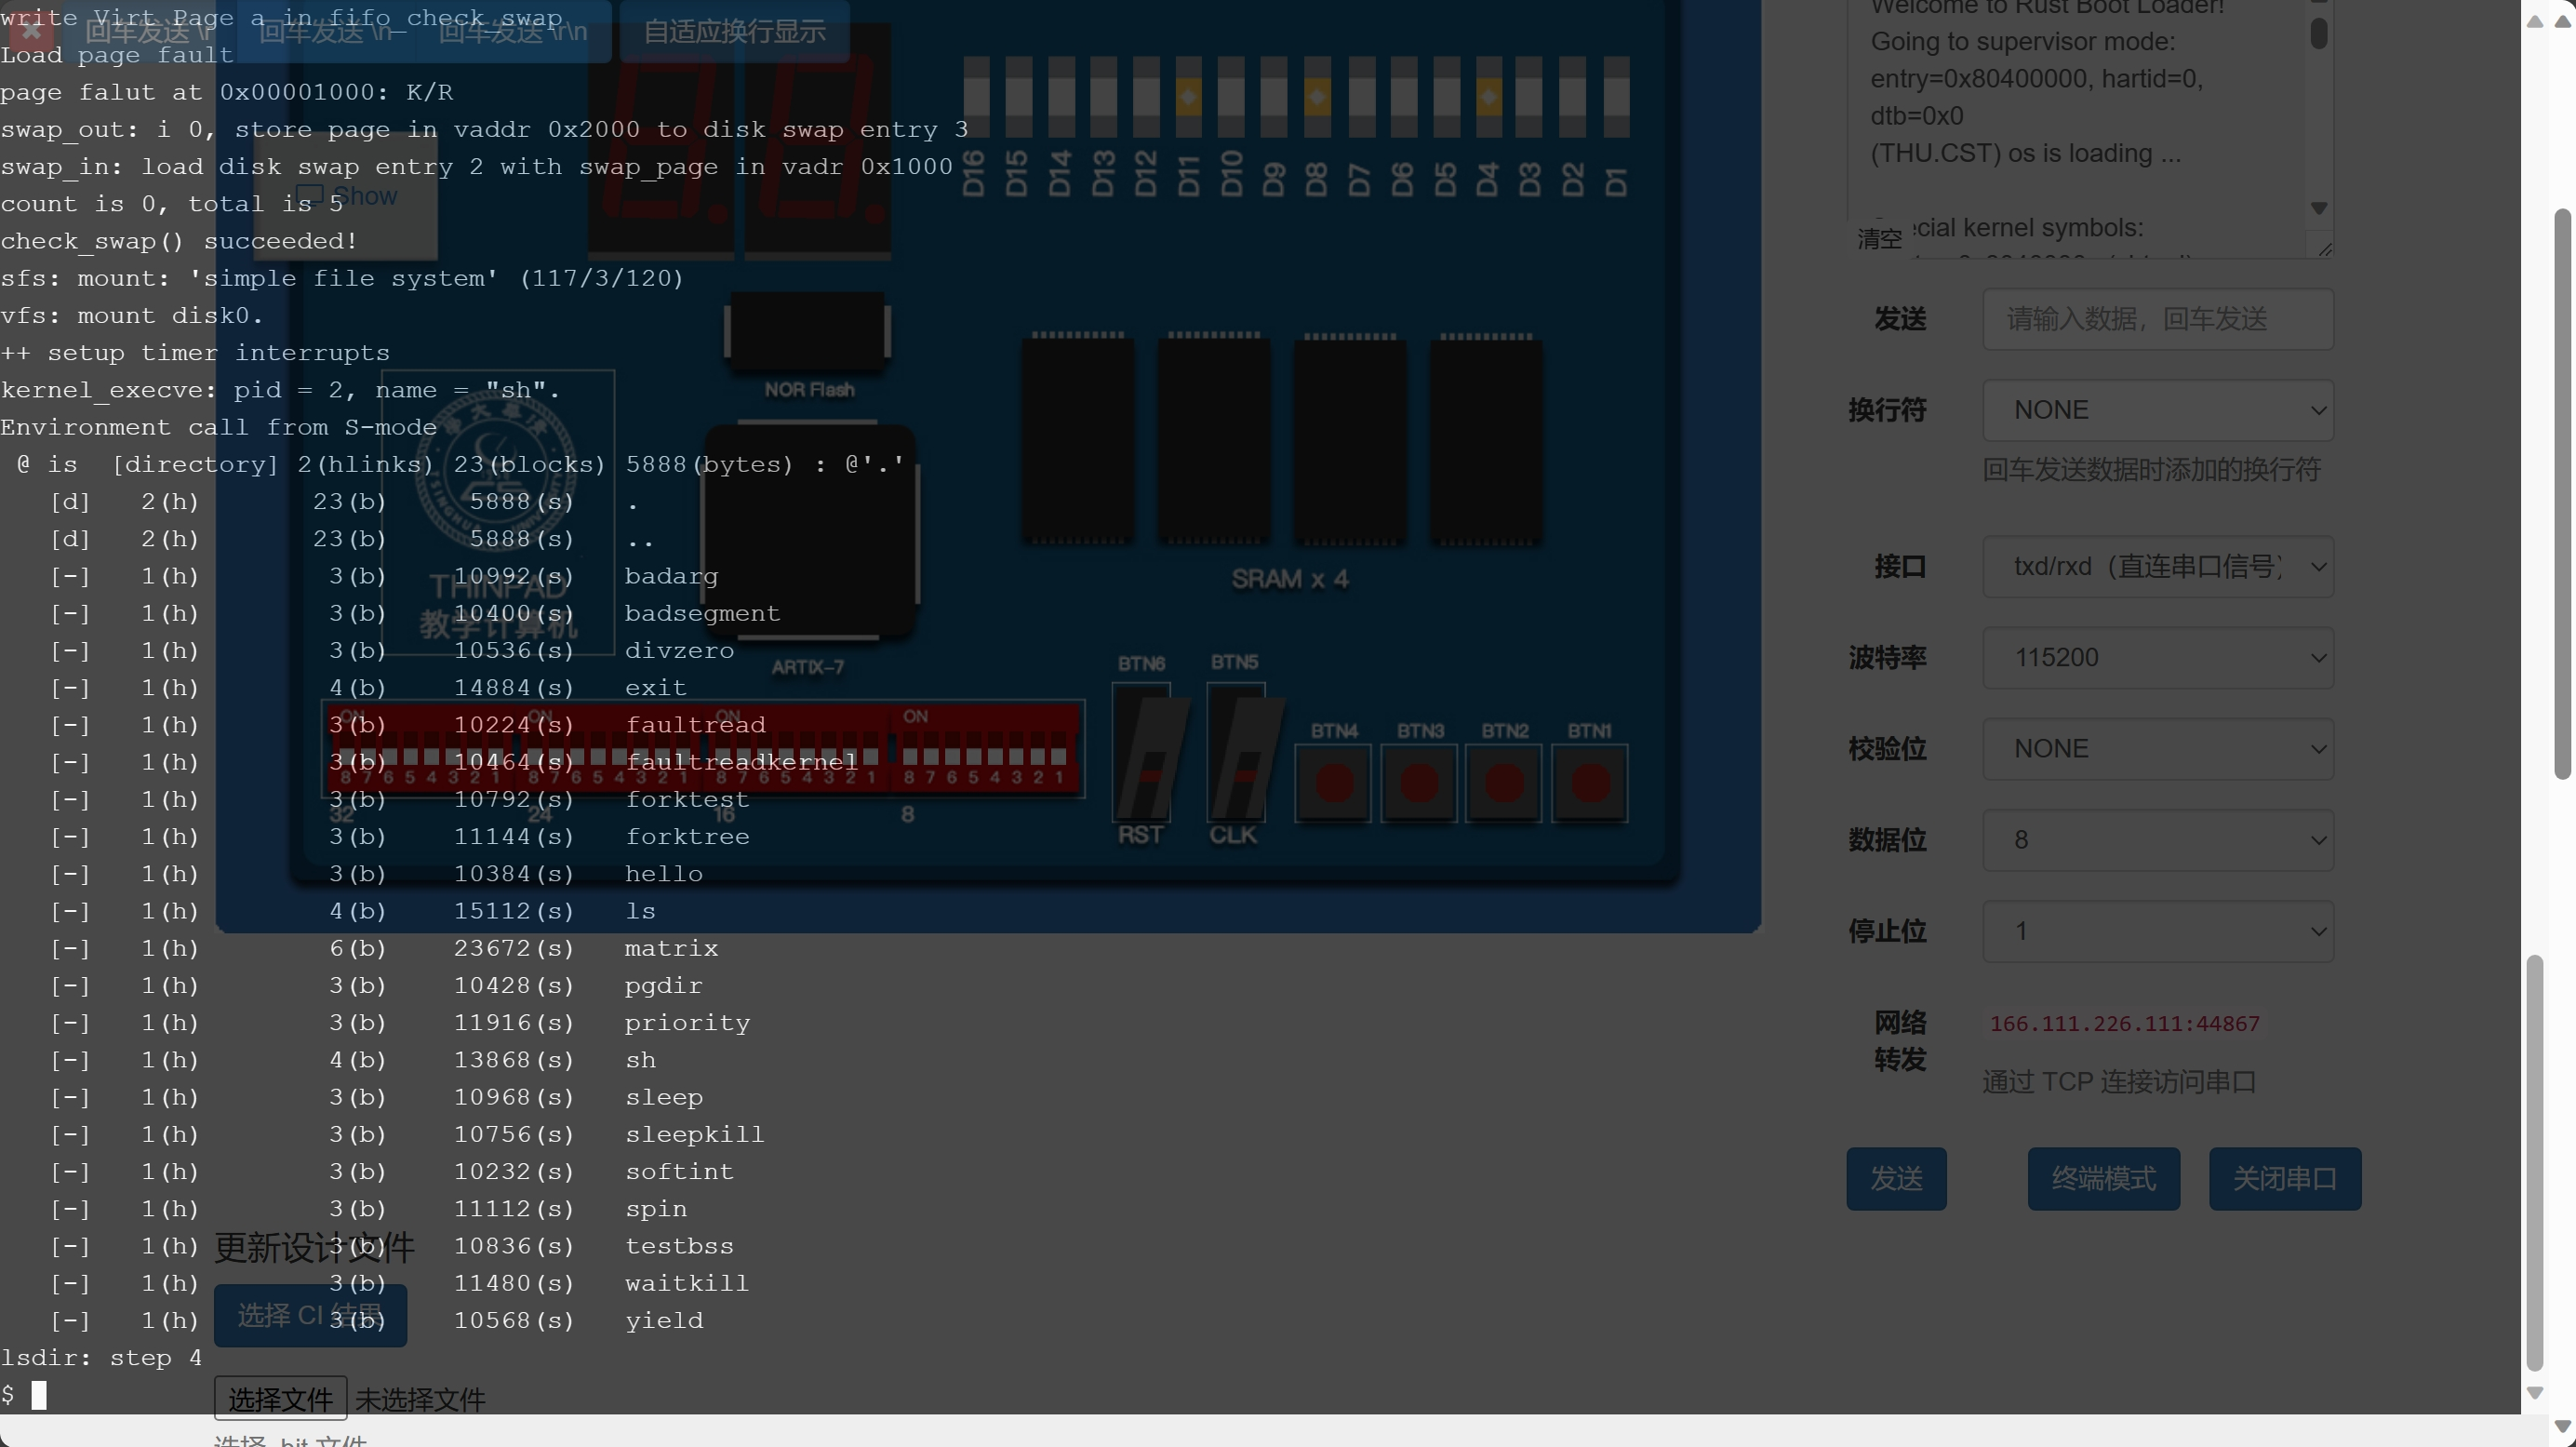
\includegraphics[scale=0.15]{assets/ucore_ls.png}
    \caption{uCore 运行截图 - ls 命令}
    \label{fig:ucore_ls}
\end{figure}

\begin{figure}[H]
    \centering
    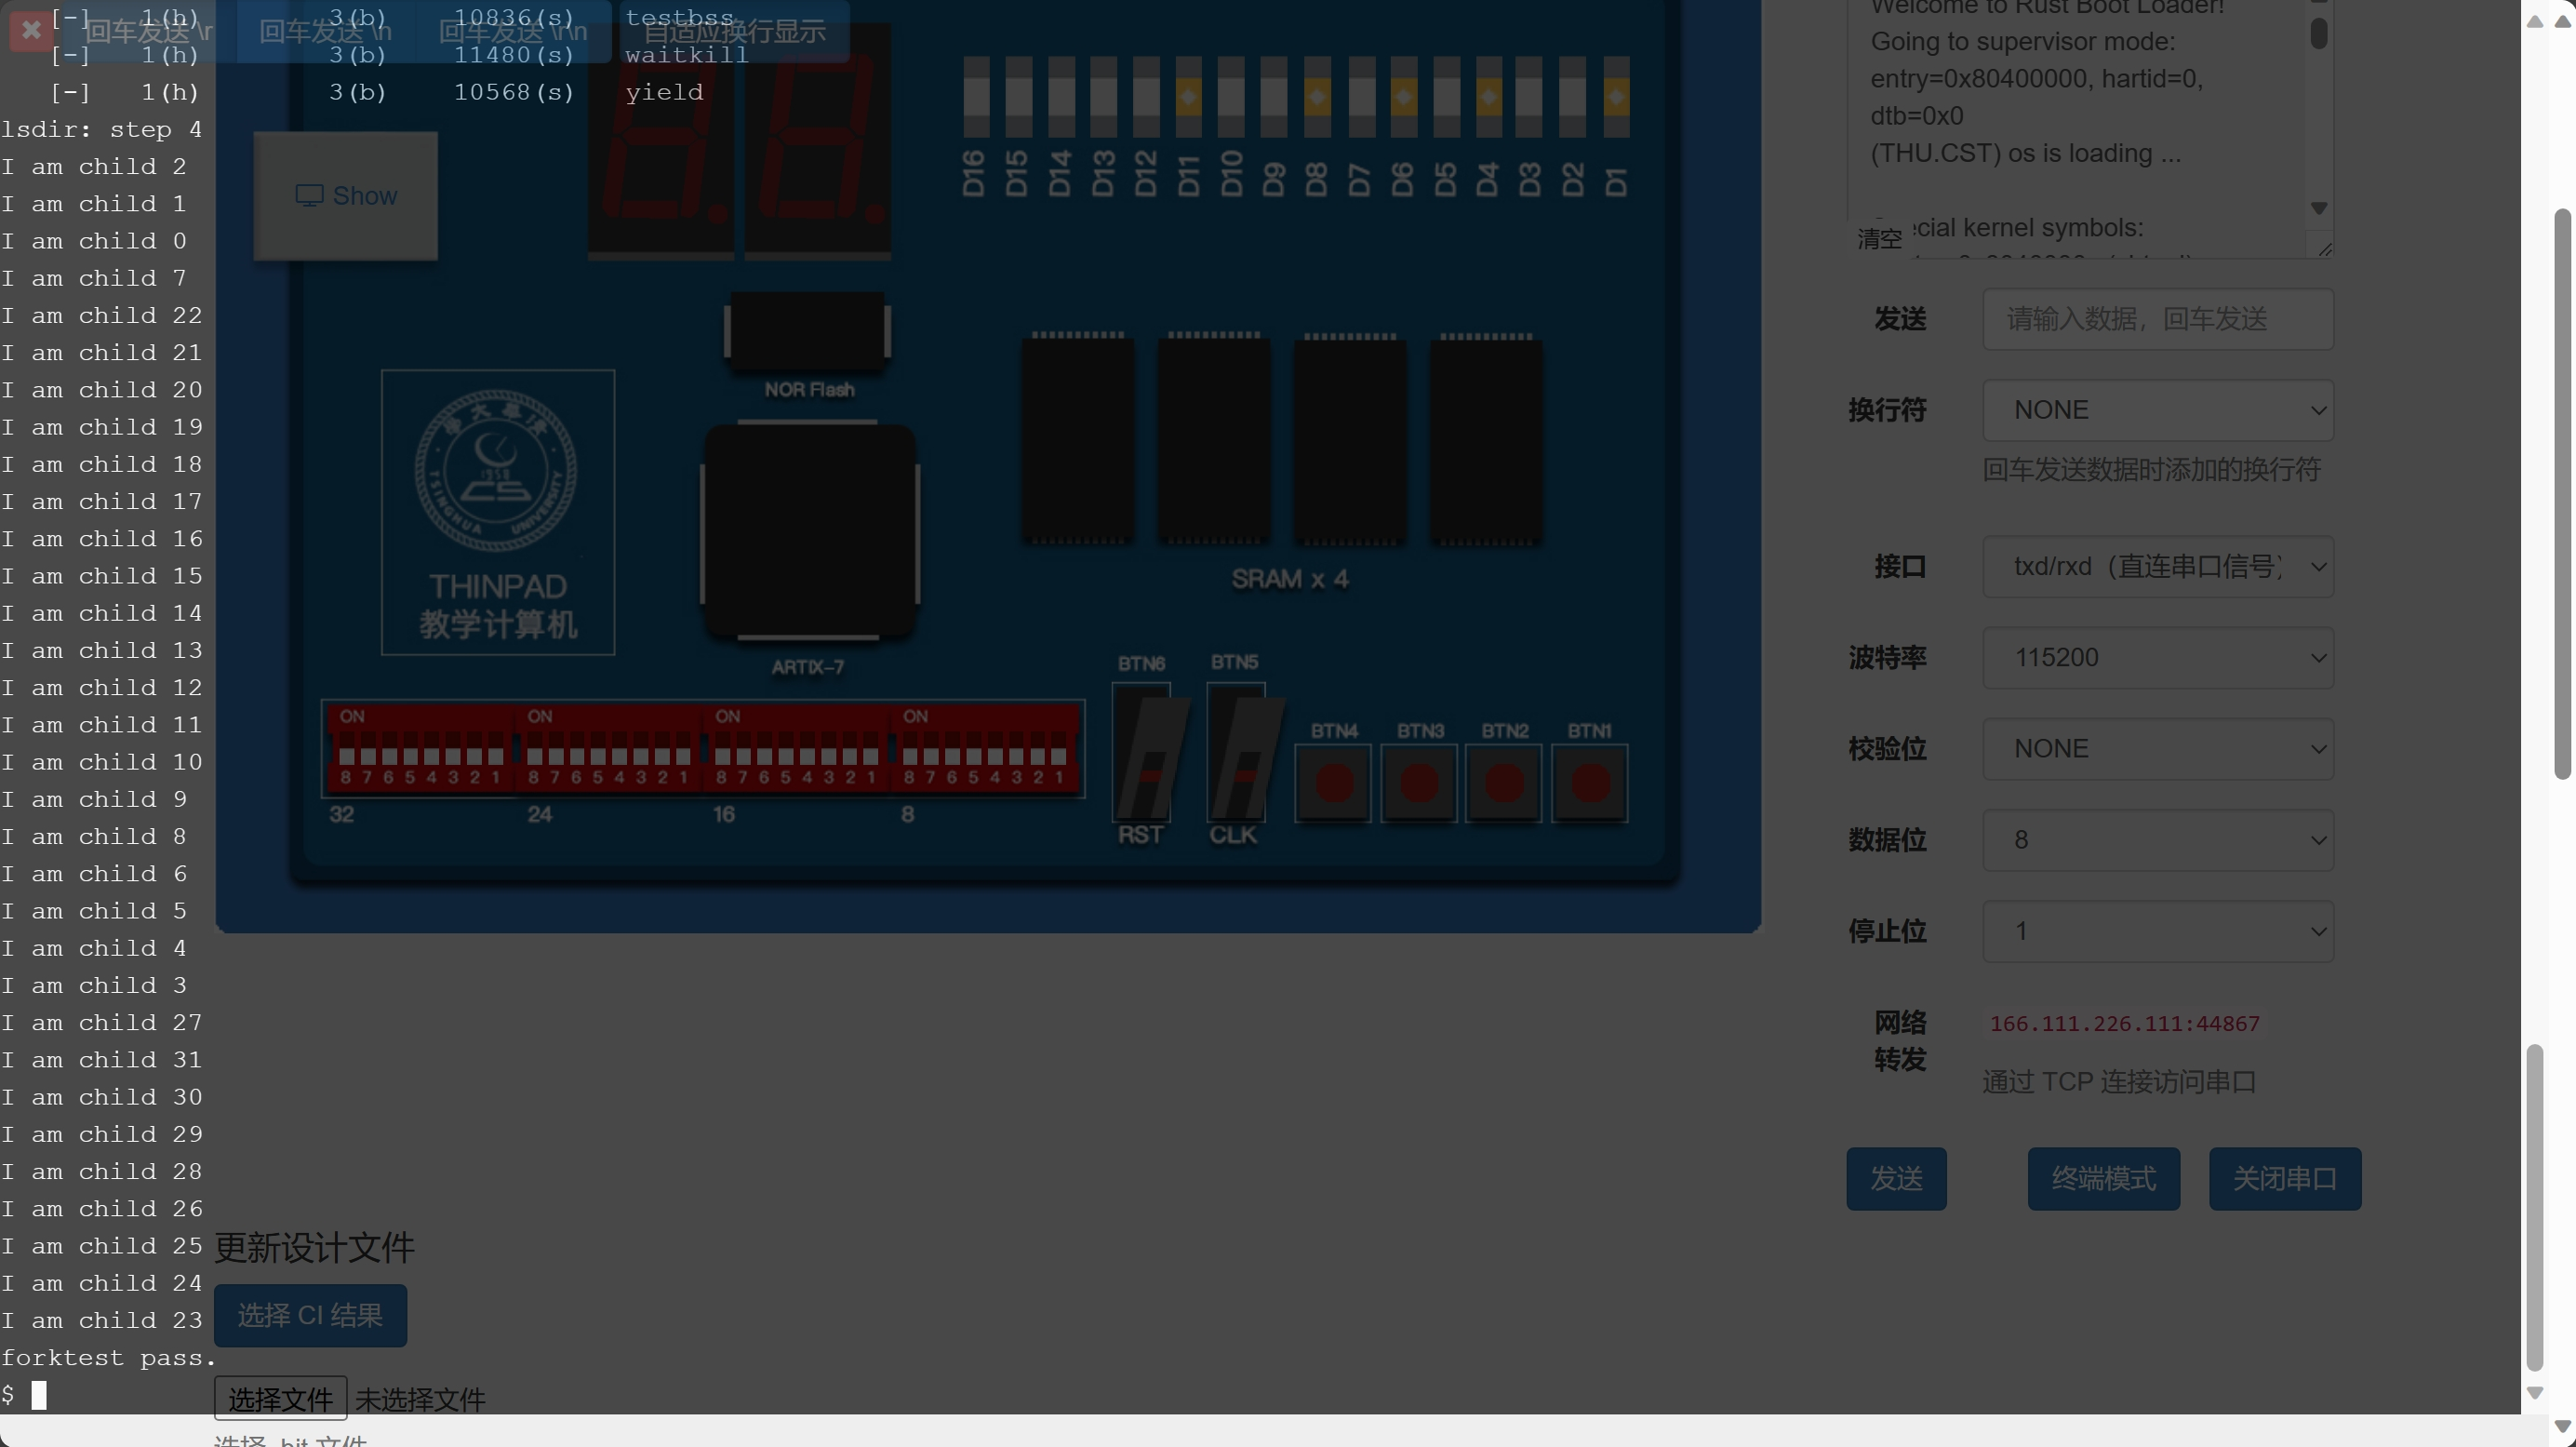
\includegraphics[scale=0.15]{assets/ucore_forktest.png}
    \caption{uCore 运行截图 - forktest 命令}
    \label{fig:ucore_forktest}
\end{figure}

\begin{figure}[H]
    \centering
    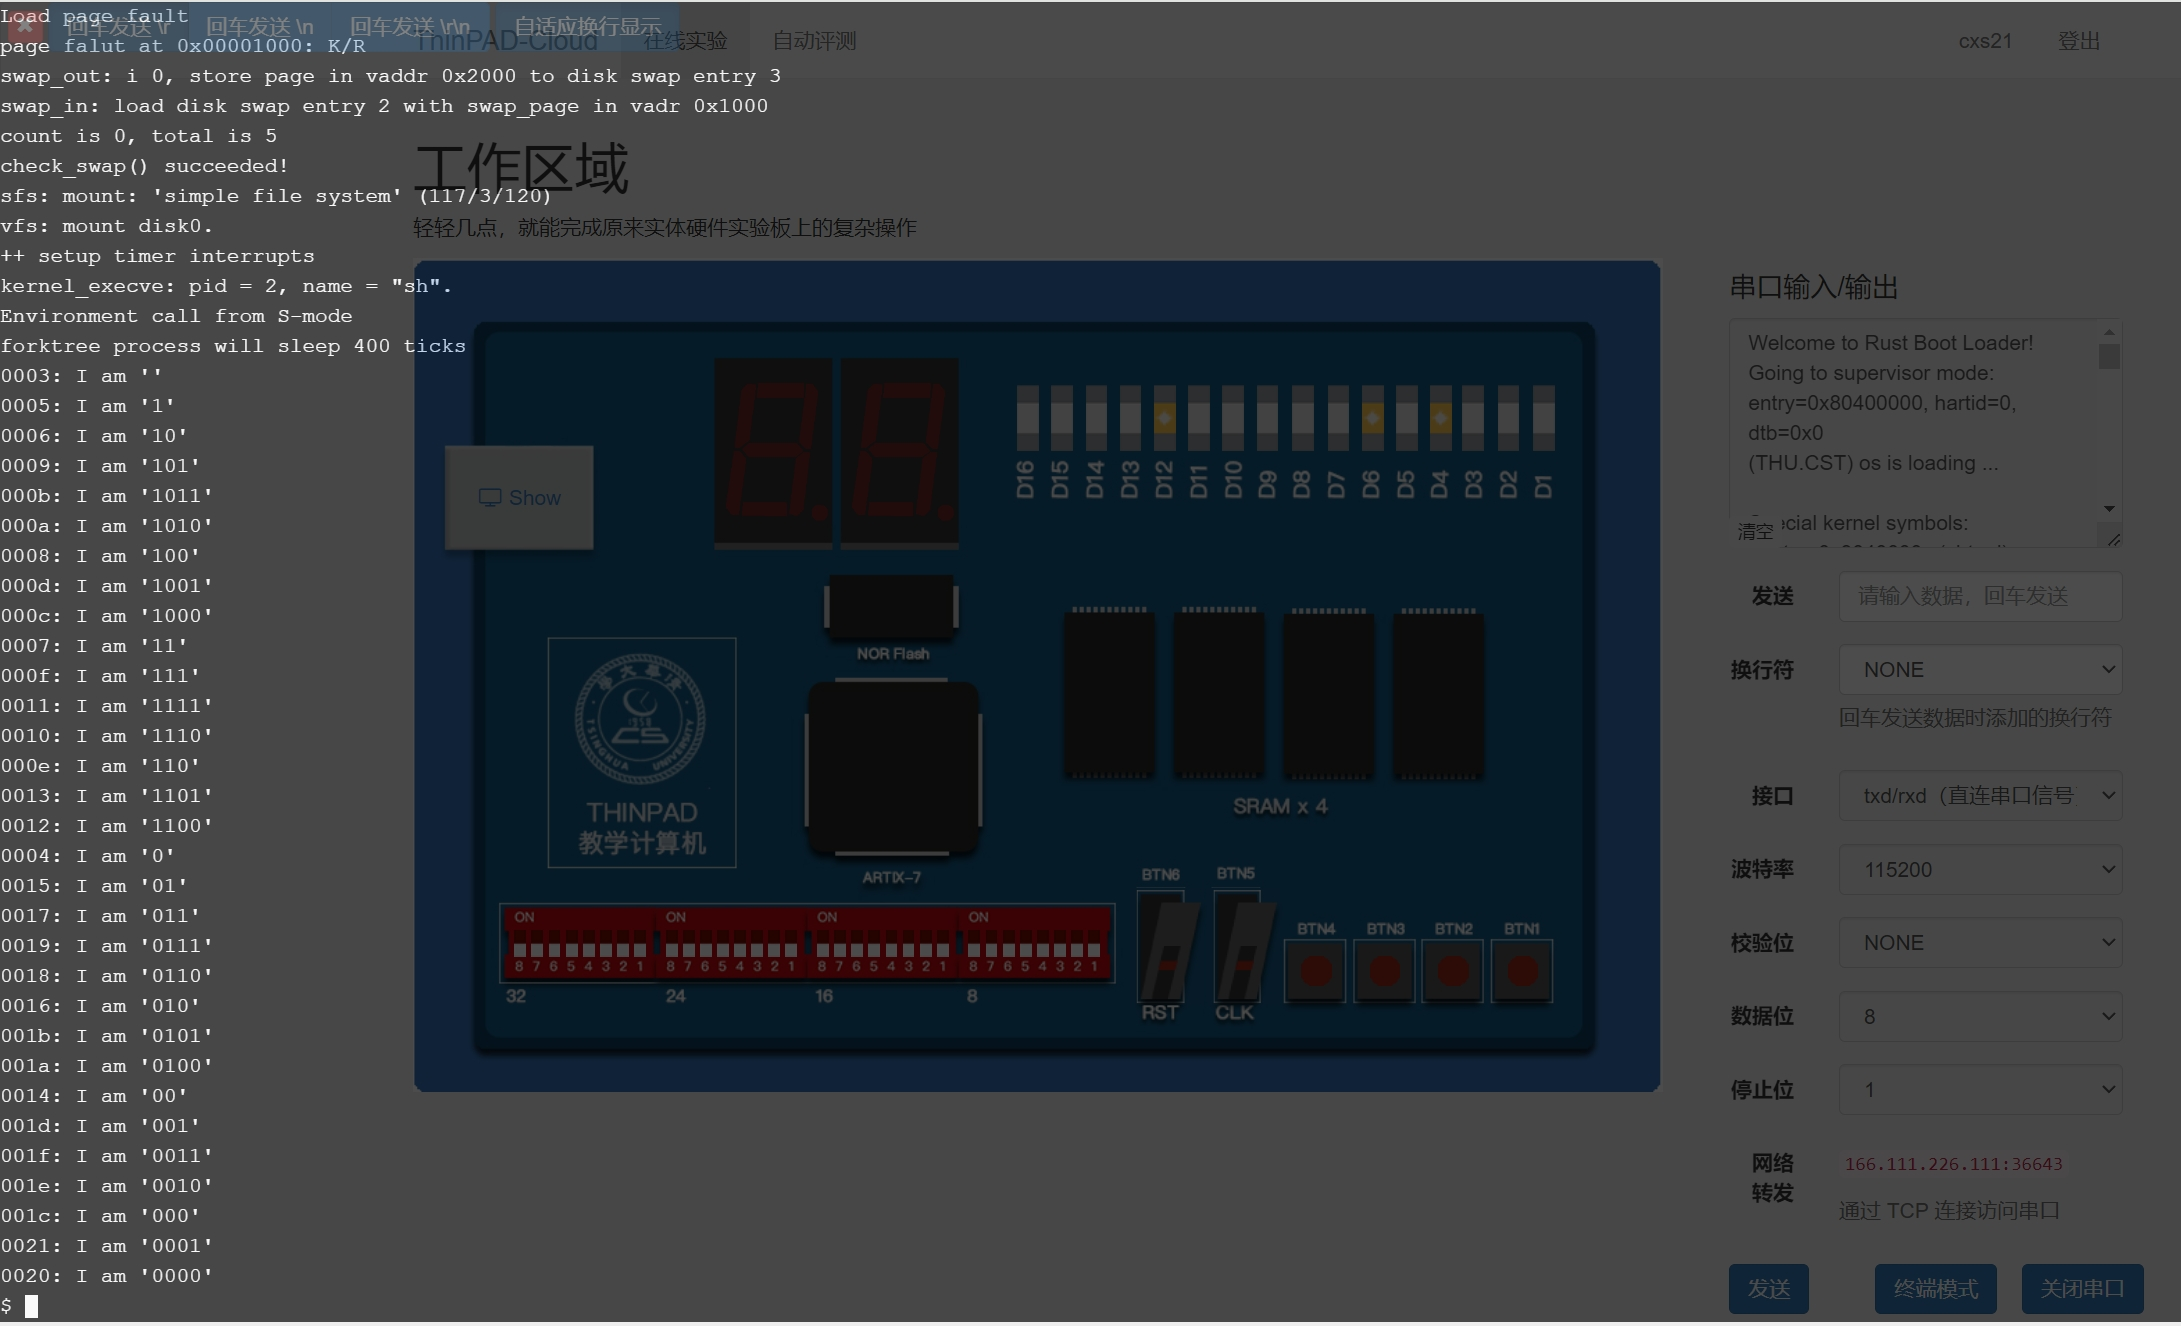
\includegraphics[scale=0.18]{assets/ucore_forktree.png}
    \caption{uCore 运行截图 - forktree 命令}
    \label{fig:ucore_forktree}
\end{figure}

\subsection{VGA 播放视频}

我们的处理器可以运行适当的用户程序,从而播放出存储于 Flash 的视频。效果截图如下,完成演示参见 \href{https://cloud.tsinghua.edu.cn/f/c547be4e479d4c779254/}{https://cloud.tsinghua.edu.cn/f/c547be4e479d4c779254/}。

\begin{figure}[H]
    \centering
    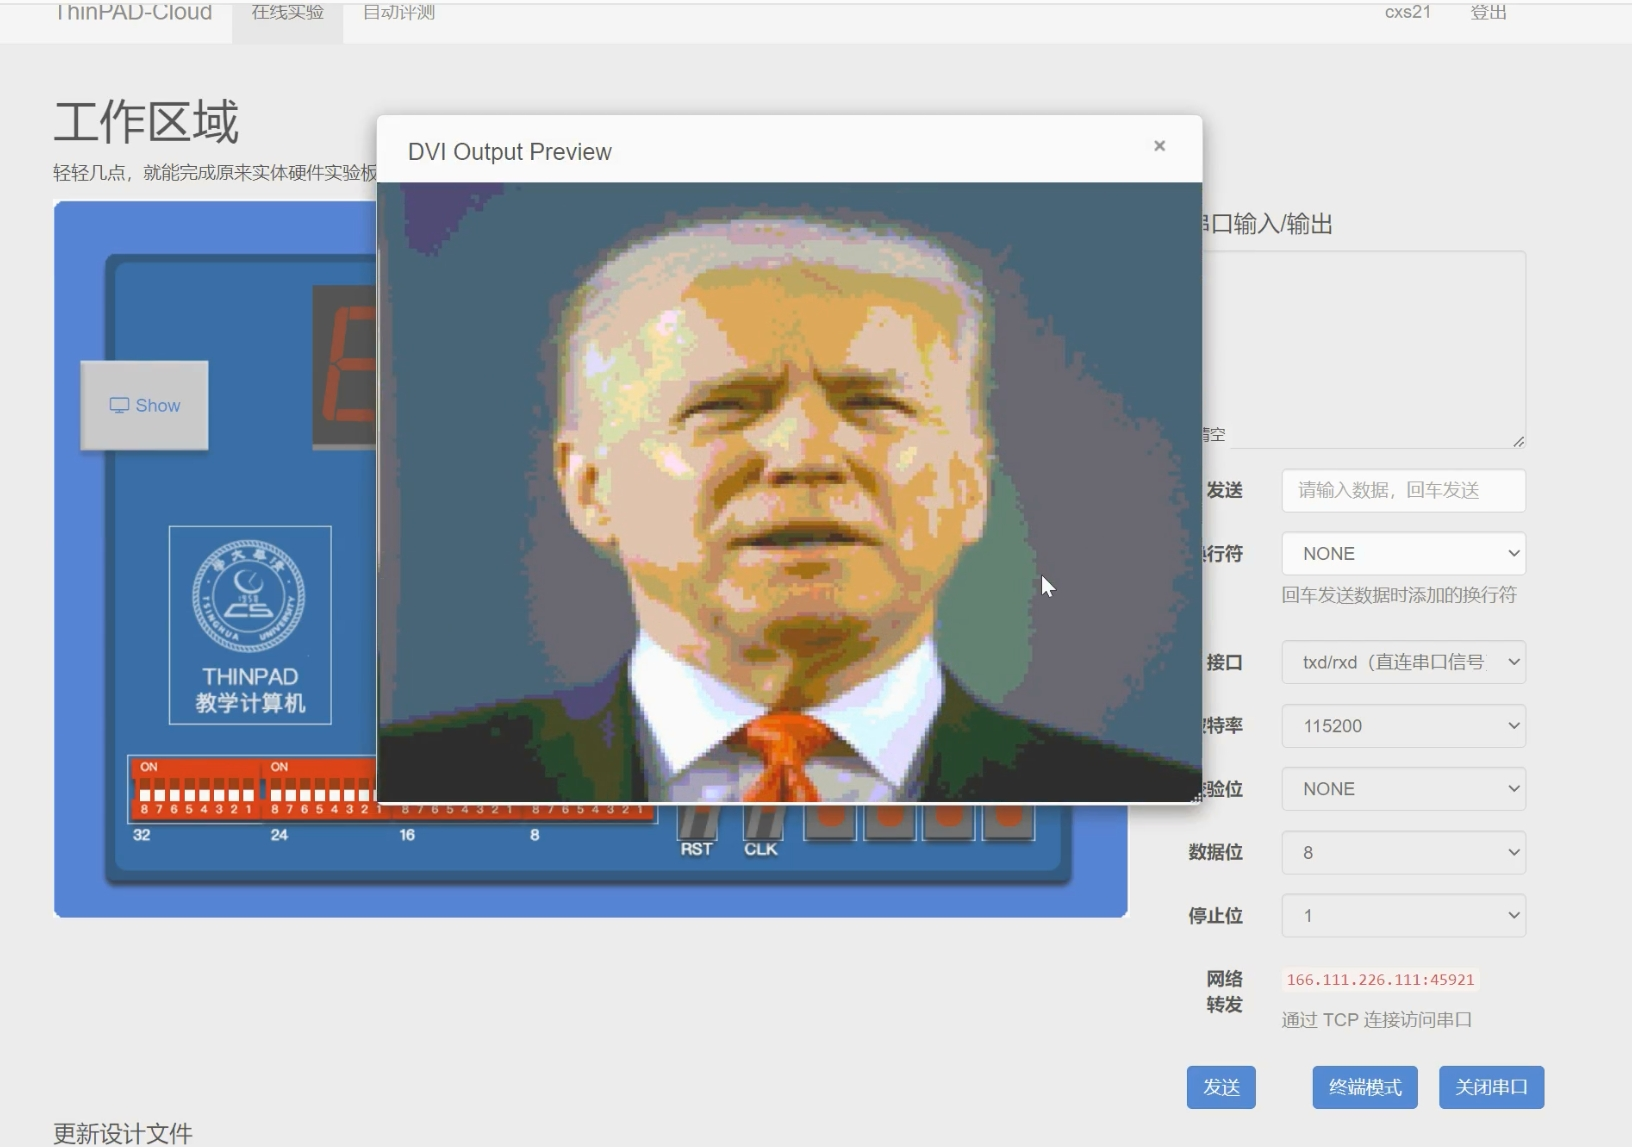
\includegraphics[scale=0.25]{assets/VGAdemo.png}
    \caption{VGA 效果演示截图}
    \label{fig:VGAdemo}
\end{figure}

\section{实验心得体会}
当然可以!在过去的三周里,我们参与了计算机组成原理造机大实验,设计并实现了一个能运行ucore操作系统的流水线cpu。这是一个既有趣又有挑战性的项目,让我深入了解了操作系统和处理器的工作原理和实现方法。最喜欢或最满意的部分是,当我们成功地让我的流水线cpu运行起来,加载并执行ucore操作系统时,我们感到了无比的兴奋和成就感。这是我们付出了三周的努力的结果,也是我们对自己的能力的证明。这是我们在计算机组成原理课程中最难忘和最有意义的经历。 % 《当然可以!》


\section{遇到的困难与解决方案}
每一步都遇到了很多困难,不一而足,主要通过仿真来解决。(“Verilog 项目都是仿真驱动开发的。” \footnote{https://lab.cs.tsinghua.edu.cn/cod-lab-docs/labs/})%引用一下出处?
% 来自:https://lab.cs.tsinghua.edu.cn/cod-lab-docs/labs/
%  Verilog 项目都是仿真驱动开发的。
% ------ 张宇翔

在增加指令时,我们使用了课程文档中提供的测例 \footnote{https://lab.cs.tsinghua.edu.cn/cod-lab-docs/labs/ex3/debug/#_5} 的 \texttt{test19} ,并结合仿真来帮助排查错误。

在调试 uCore 时,由于 uCore 本身启动需要相当长的时间(对于仿真而言),因此我们选择了上板 + ILA 的方式观测信号。

但通过 ILA 只能观测到信号首次与预期不一致时的情况(即 Error),而这不一定能暴露出代码中的 Fault,因为 ILA 能观测的信号数量和时间有限,并且我们也没有标准的(可用于对拍的)内部信号变化情况。因此我们还是基于 ILA 观测提供的线索,通过 code review 找出问题所在。

使用宏和 \texttt{localparam, parameter} 代替硬编码的常数,可以避免相当一部分错误。

\section{思考题}
% 第 4 题及以后的思考题仅在你实现了括号中的相应扩展功能时才需要完成。

\begin{itemize}
    \item 流水线 CPU 设计与多周期 CPU 设计的异同?插入等待周期(气泡)和数据旁路在处理数据冲突的性能上有什么差异。
    
    \textbf{答}:(1)异:流水线 CPU(在未发生冲突时)每一时钟周期可以同时处理多条指令(每一流水段各处理一条指令),而多周期 CPU 每一时钟周期只在处理一条指令;流水线 CPU 的每个周期都可以进、出一条指令(假设每个流水段都可以在一周期完成的话),多周期 CPU 需要多个周期才能进、出一条指令。
    
    (2)同:每条指令都需要经过多个周期才能完成执行。

    (3)加入数据旁路后,可以解决相当一部分数据冲突,尽早获得部分寄存器更新后的值,而不需要等到它写回寄存器后才能获得。因此,可以避免很多气泡的插入,从而使得性能得到一定提升。
    
    \item 如何使用 Flash 作为外存,如果要求 CPU 在启动时,能够将存放在 Flash 上固定位置的监控程序读入内存,CPU 应当做什么样的改动?
    
    \textbf{答}:首先,需要完成 Flash 控制器,并为 Flash 分配相应的地址区间和修改 wishbone slave mux,这些已在本实验中完成。然后,将 CPU 的起始 PC 修改为在 Flash 上固定位置的监控程序的起始地址即可。
    
    \item 如何将 DVI 作为系统的输出设备,从而在屏幕上显示文字?
    
    \textbf{答}:首先,需要为 DVI 分配一块内存(例如使用 Block RAM 等),控制器以一定的频率不断地读取这些数据并发送到  DVI 设备上。然后,将文字转换为点阵图像,并向显存的地址写入该图像。
    
    \item (分支预测)对于性能测试中的 3CCT 测例,计算一下你设计的分支预测在理论上的准确率和性能提升效果,和实际测试结果对比一下是否相符。
    
    \textbf{答}:由于我们的分支预测加入了有效位机制,所以在第一次遇到 bne , j 跳转指令时不会跳转,实际上是需要跳转;最后一次预测需要跳转,实际上不需要,这是两类失误。
    跳转指令一共出现了 $3\times 67108664+1$ 次,失败 4 次,命中率 $99\%$,命中后不需要冲刷流水线,少插入3条空指令,耗时约为原来的 4/7。
    
    实际结果测试中(参见 \ref{performance}), 3CCT 测例的性能从 67.109s 提升到 26.837s,与理论估计较相近。 % 与理论估计偏差很大啊 qaq... 因为还有指令缓存等其他因素影响,比如下道题,没有dcache也有提升,就是因为icache,可以参照下道题看看
    % 26.837/67.109 = 0.3999,
    % 4/7 = 0.5714,3/7 = 0.4286
    
    % \item (缓存)对于性能测试中的 4MDCT 测例,计算一下你设计的缓存在理论上的命中率和性能提升效果,和实际测试结果对比一下是否相符。
    
    % \textbf{答}:
    
    \item (虚拟内存)考虑支持虚拟内存的监控程序。如果要初始化完成后用 G 命令运行起始物理地址 0x80100000 处的用户程序,可以输入哪些地址?分别描述一下输入这些地址时的地址翻译流程。
    
    \textbf{答}:0x80100000 或 0x0000000。用 term 连接监控程序后,使用 \texttt{T} 命令查看页表,结果节选如下。
    
    \begin{lstlisting}[
        numbers=left,
        frame=single,           % 添加边框
        basicstyle=\fontsize{8}{10}\selectfont, % 设置全局字号
        lineskip=4pt,           % 设置行距
        tabsize=4,              % 设置制表符的宽度为4个空格
        % xleftmargin=15pt,       % 设置左侧缩进的距离为15pt
        caption={监控程序页表(节选)} % 标题
    ] 
    Page table at 80002000
     Virtual Address     |      Physical Address     | D | A | G | U | X | W | R | V
    00000000-00000fff          80100000-80100fff       1   1   1   1   1   0   1   1
    ...
    80100000-80100fff          80100000-80100fff       1   1   1   1   1   0   1   1
    \end{lstlisting}

    可见使用 0x80100000 或 0x0000000 都可以对应到物理地址 0x80100000 处的用户程序。而虚拟地址结构如下:
    \begin{lstlisting}[
        numbers=left,
        frame=single,           % 添加边框
        basicstyle=\fontsize{8}{10}\selectfont, % 设置全局字号
        lineskip=4pt,           % 设置行距
        tabsize=4,              % 设置制表符的宽度为4个空格
        % xleftmargin=15pt,       % 设置左侧缩进的距离为15pt
        caption={虚拟地址结构} % 标题
    ] 
        virtual address:
      |       VPN (virtual page number)     | offset |
      |        VPN1       |       VPN0      |        |
      |         10        |        10       |   12   |
      |  0b 10 0000 0000  | 0b 01 0000 0000 | 0x000  | 0x80100000
      |  0b 00 0000 0000  | 0b 00 0000 0000 | 0x000  | 0x00000000
    \end{lstlisting}
    
    在 PC 切换到这些输入地址后,首先会查询 \texttt{(satp.ppn << 12) + (vaddr.vpn1 << 2)} 处的第一级页表项(即第一级页表的第 \texttt{0x200, 0x000} 项),然后查询 \texttt{(\{lv1\_pte.ppn1, lv1\_pte.ppn0\} << 12) + (vaddr.vpn0 << 2)} 处的第二级页表项(即第一级页表的第 \texttt{0x100, 0x000} 项)。
    
    查询得到相应的 PPN,然后拼接上 \texttt{offset} 得到物理地址。

    \item (异常与中断)假设第 a 个周期在 ID 阶段发生了 Illegal Instruction 异常,你的 CPU 会在周期 b 从中断处理函数的入口开始取指令执行,在你的设计中,b - a 的值为?
    
    \textbf{答}:该指令会继续执行 EXE、MEM1,到达 MEM2 阶段之后进入异常处理入口,b-a=4.
\end{itemize}

\end{document}
